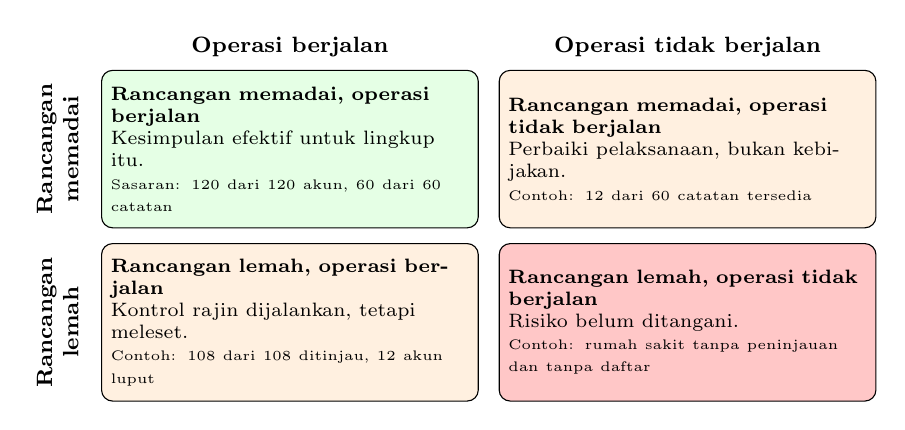
\begin{tikzpicture}[
  font=\scriptsize,
  sel/.style={draw, rounded corners, align=left, text width=4.55cm, minimum height=2cm},
  judul/.style={font=\footnotesize\bfseries, align=center}]
  \node[sel, fill=green!10] (a) at (0,0)
    {\textbf{Rancangan memadai, operasi berjalan}\\Kesimpulan efektif untuk lingkup itu.
    \\{\tiny\mdseries Sasaran: 120 dari 120 akun, 60 dari 60 catatan}};
  \node[sel, fill=orange!12] (b) at (5.05,0)
    {\textbf{Rancangan memadai, operasi tidak berjalan}\\Perbaiki pelaksanaan, bukan kebijakan.
    \\{\tiny\mdseries Contoh: 12 dari 60 catatan tersedia}};
  \node[sel, fill=orange!12] (c) at (0,-2.2)
    {\textbf{Rancangan lemah, operasi berjalan}\\Kontrol rajin dijalankan, tetapi meleset.
    \\{\tiny\mdseries Contoh: 108 dari 108 ditinjau, 12 akun luput}};
  \node[sel, fill=red!22] (d) at (5.05,-2.2)
    {\textbf{Rancangan lemah, operasi tidak berjalan}\\Risiko belum ditangani.
    \\{\tiny\mdseries Contoh: rumah sakit tanpa peninjauan dan tanpa daftar}};
  \node[judul] at (0,1.3) {Operasi berjalan};
  \node[judul] at (5.05,1.3) {Operasi tidak berjalan};
  \node[judul, rotate=90] at (-2.95,0) {Rancangan\\memadai};
  \node[judul, rotate=90] at (-2.95,-2.2) {Rancangan\\lemah};
\end{tikzpicture}
